\def\SCALE{.85}
\begin{tikzpicture}[,scale=\SCALE,font=\sffamily\fontsize{8}{8}\selectfont]
  \def\WDTA{3in}
  \def\WDTB{2in}
  \def\WDTC{2.35in}
  \def\WDTD{3in}
  \def\DCOL{black!8}
  \def\DCOLS{black}
  \def\ECOLA{black!5}
  \def\ECOLB{black!5}
  \def\ECOLC{Green4!5}
  \def\ECOLD{Green4!5}
  \def\LWD{2pt}
  \def\LWDA{6pt}
  \def\ACOL{black}
  \def\OPC{.7}
  \def\OPCA{.95}
  \def\OPCB{.15}
  \def\CIRC{circle}
  \clip (3.25in,0.02in) rectangle (-4.1in,-8.95in);
  \node[] (N0) at (0,0) {};
 
\node[anchor=north east] (N1) at ([xshift=.75in,yshift=0in]N0.north west) {
%
  \begin{tikzpicture}[anchor=east,scale=\SCALE,]
\tikzset{xcirc/.style={circle,fill=\ECOLB,opacity=\OPC,rounded corners=5pt,draw=\DCOL,line width=\LWD,scale=\SCALE}}
\tikzset{xcircs/.style={circle,fill=none,opacity=1,rounded corners=5pt,draw=none,ultra thick,,scale=\SCALE}}
\tikzset{xdr/.style={\ACOL,line width=\LWDA, opacity=\OPCA}}
    \node[xcirc,inner sep=-12pt,label={[yshift=.5in,distance=-.75in,align=center]-90:Predictor for\\index 1274}] (P1274) at (0,0) {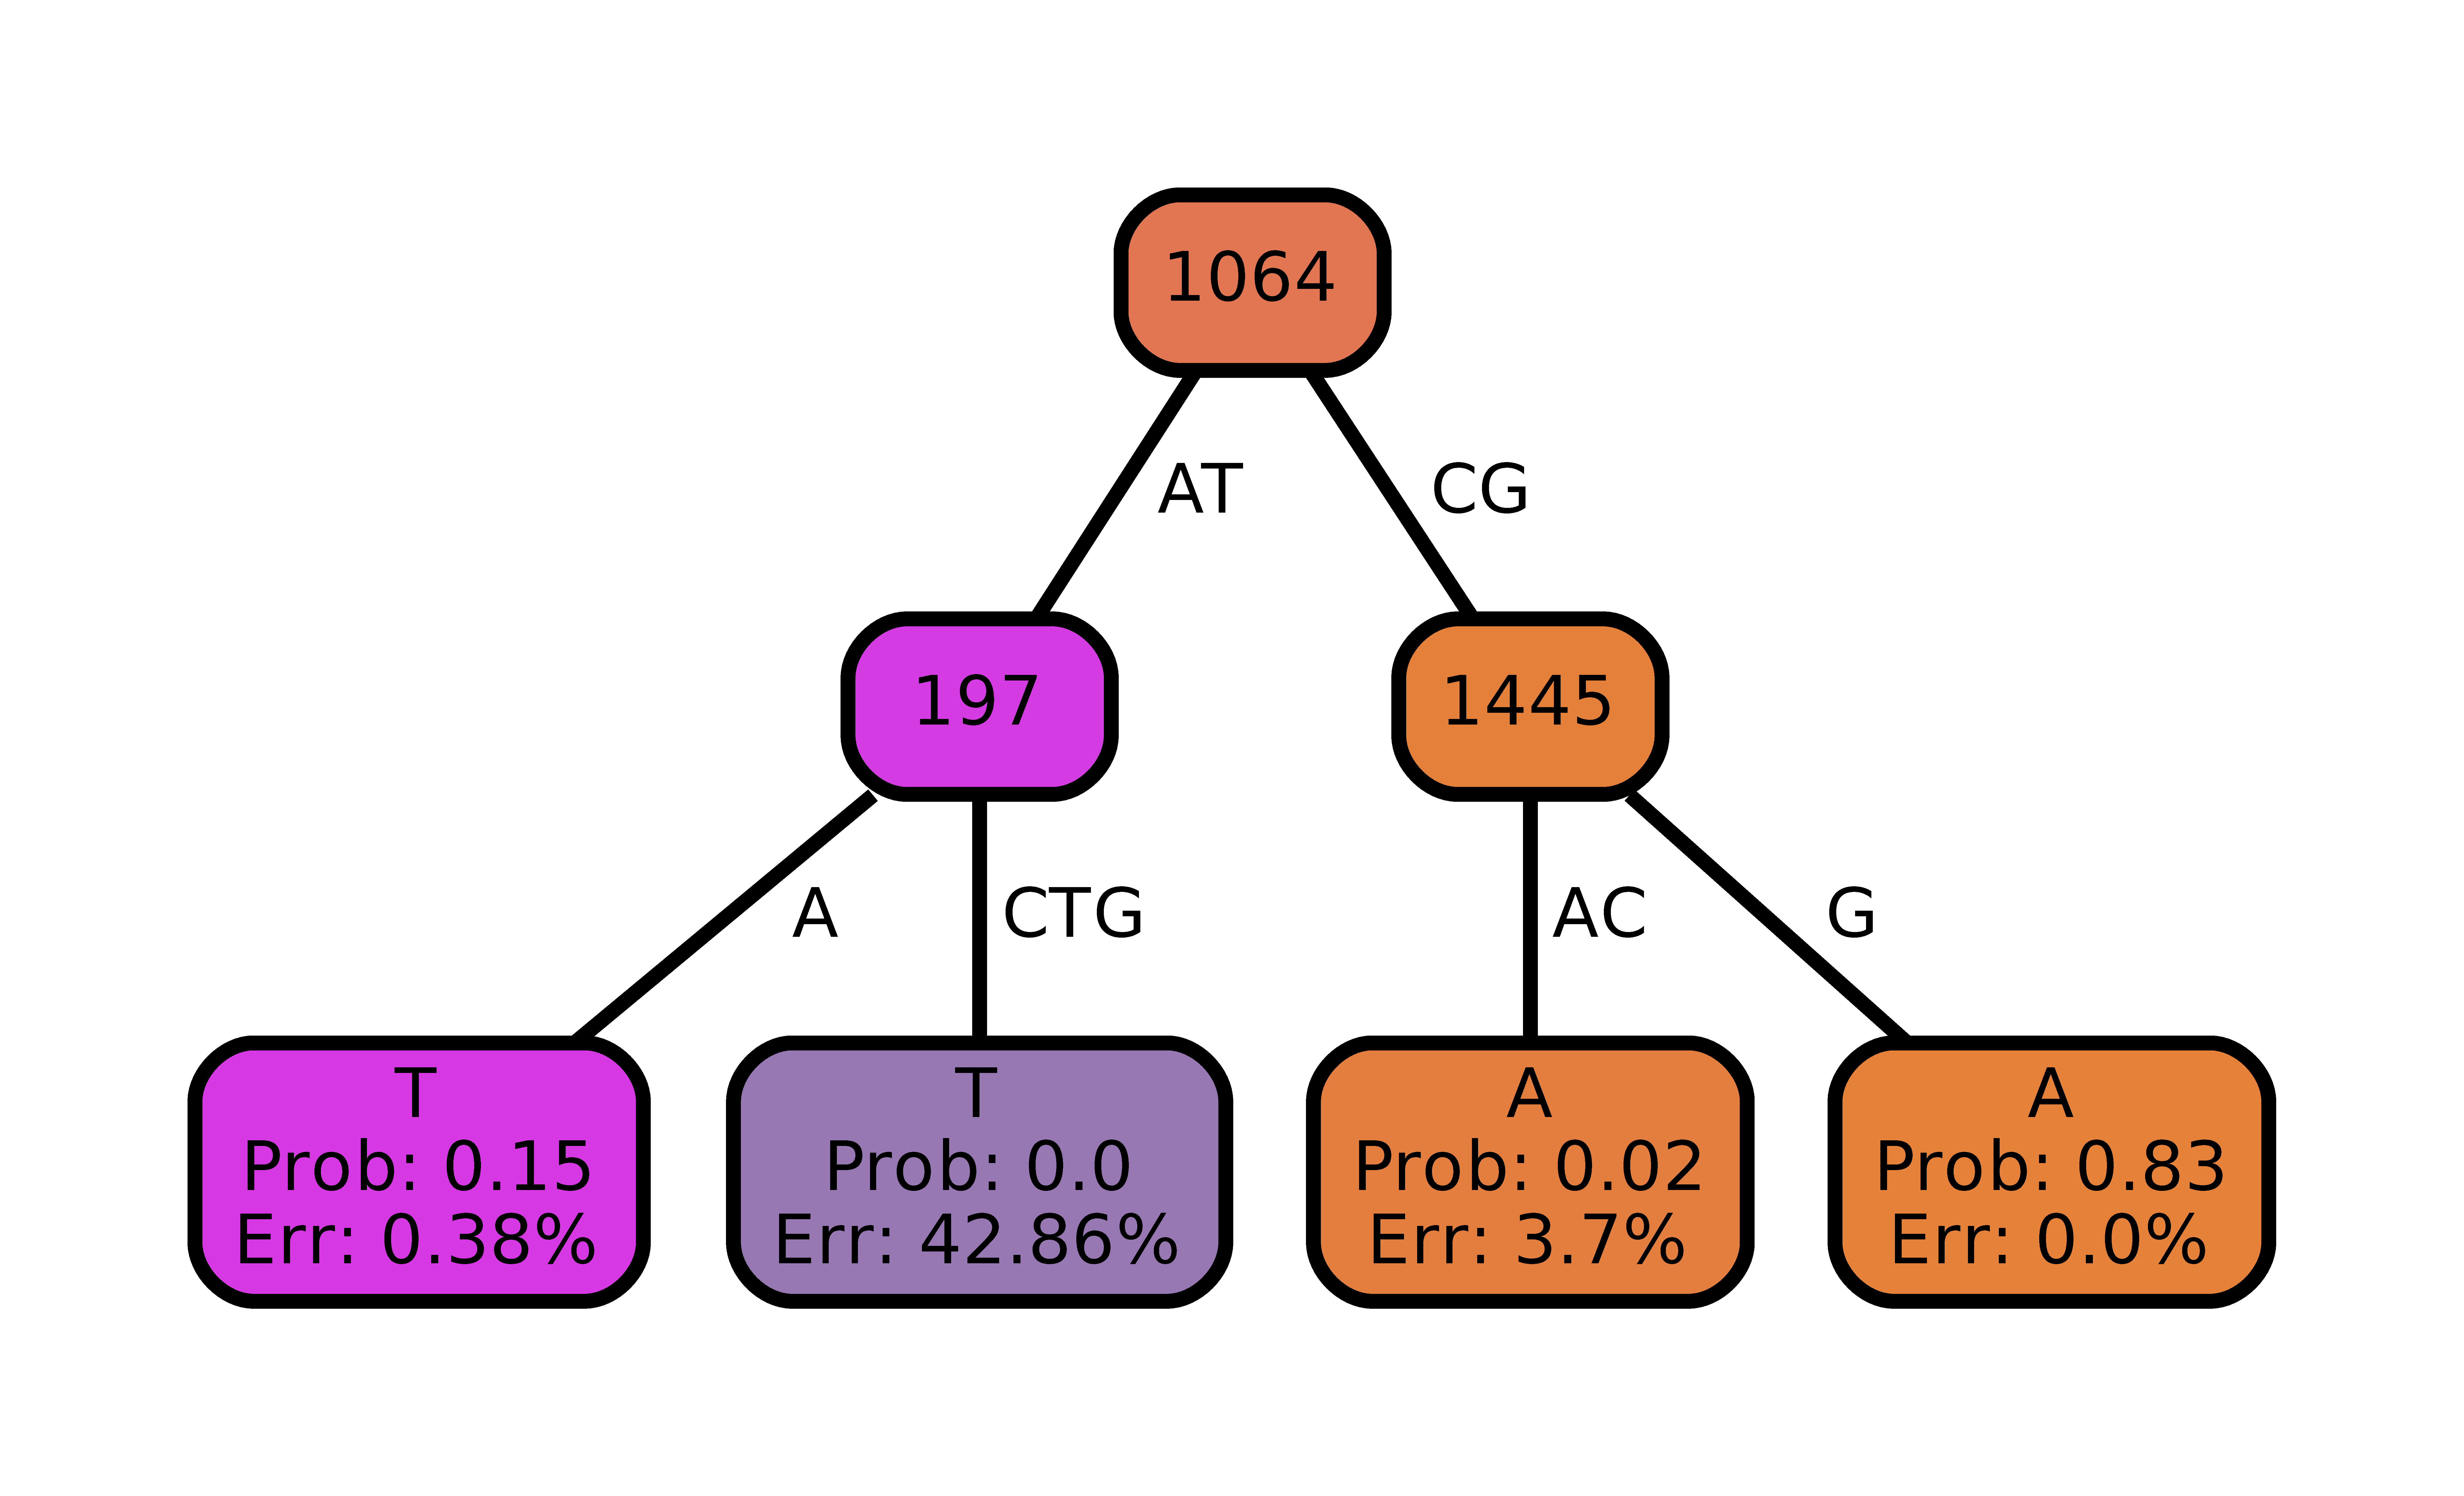
\includegraphics[width=\WDTA]{Figures/plotdata/TREE_P1274}};
    \node[xcirc,inner sep=-12pt,anchor=south,label={[yshift=.35in,distance=-.75in,align=center]-90:Predictor for\\index 1064}] (P1064) at ([xshift=1.5in,yshift=-.75in]P1274.north) {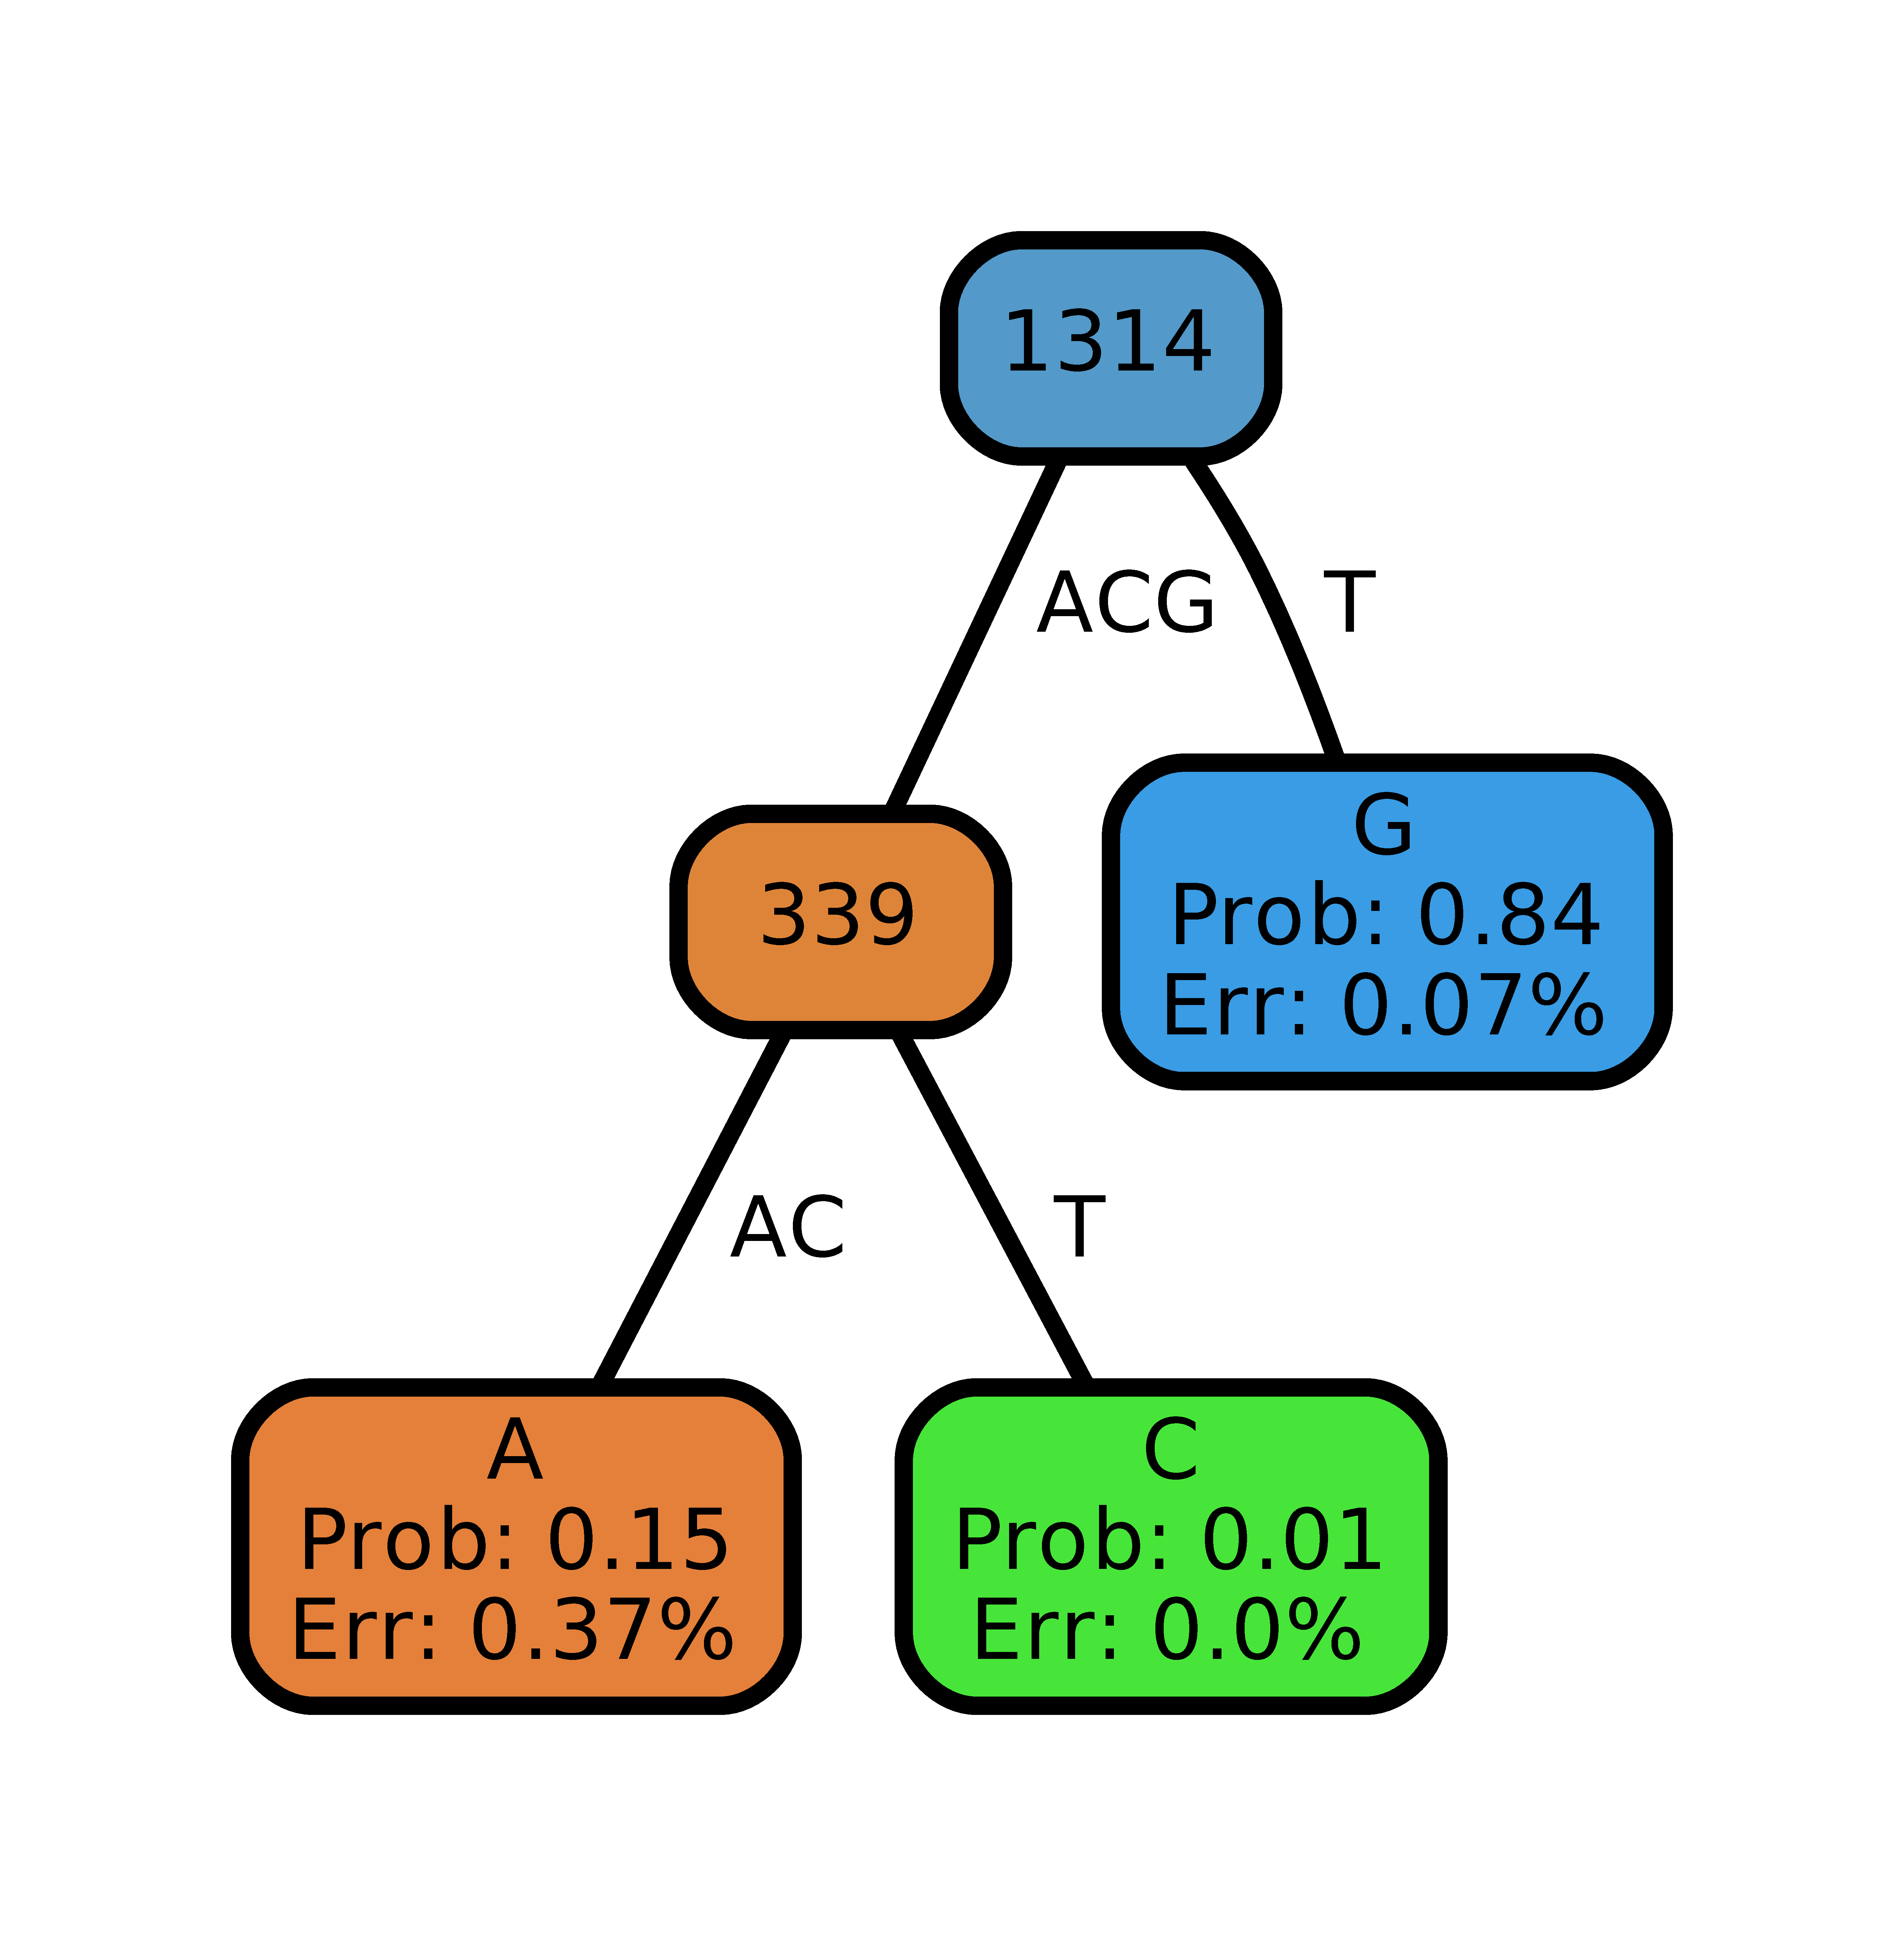
\includegraphics[width=\WDTB]{Figures/plotdata/TREE_P1064}};
     \node[xcirc,inner sep=-17pt,anchor=east,label={[xshift=.75in,yshift=.25in,distance=-.75in,align=center]-145:Predictor for\\index 1314}] (P1314) at ([xshift=.3in,yshift=.65in]P1064.west) {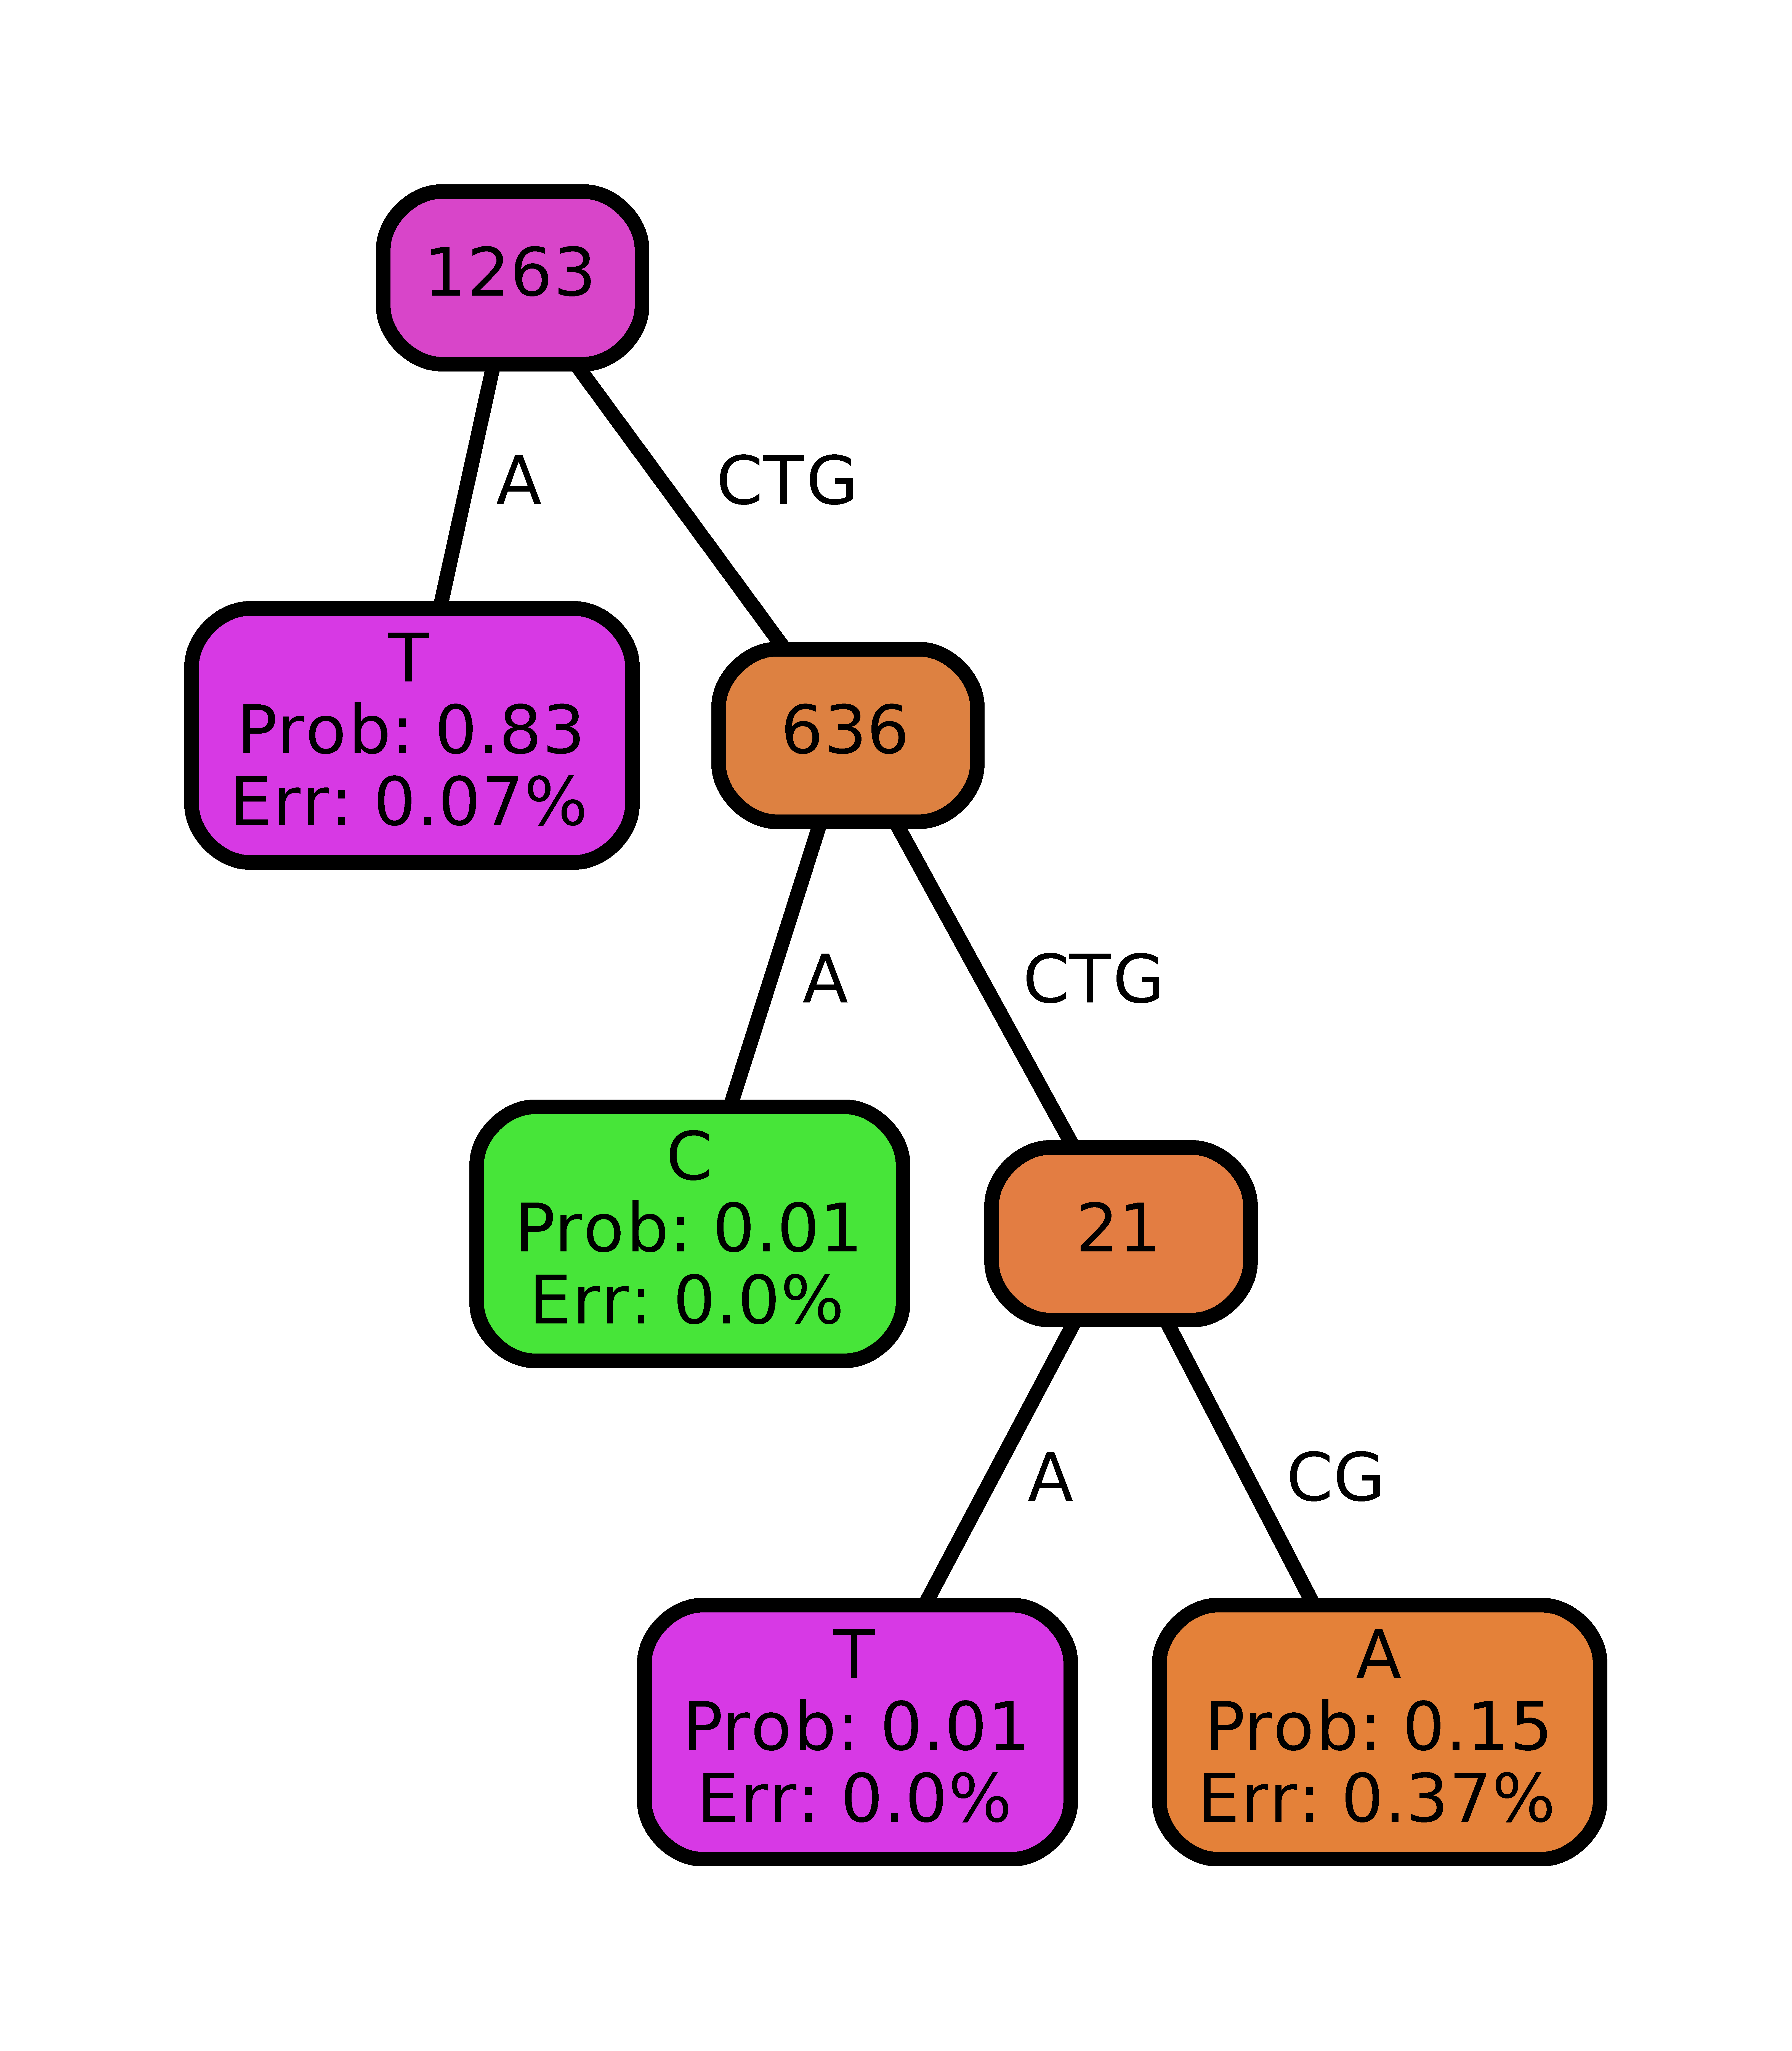
\includegraphics[width=\WDTC]{Figures/plotdata/TREE_P1314}};
     \node[xcirc,inner sep=-12pt,anchor=south west,label={[yshift=.5in,distance=-.75in,align=center]-90:Predictor for\\index 1263}] (P1263) at ([xshift=-.35in,yshift=-.4in]P1314.north east) {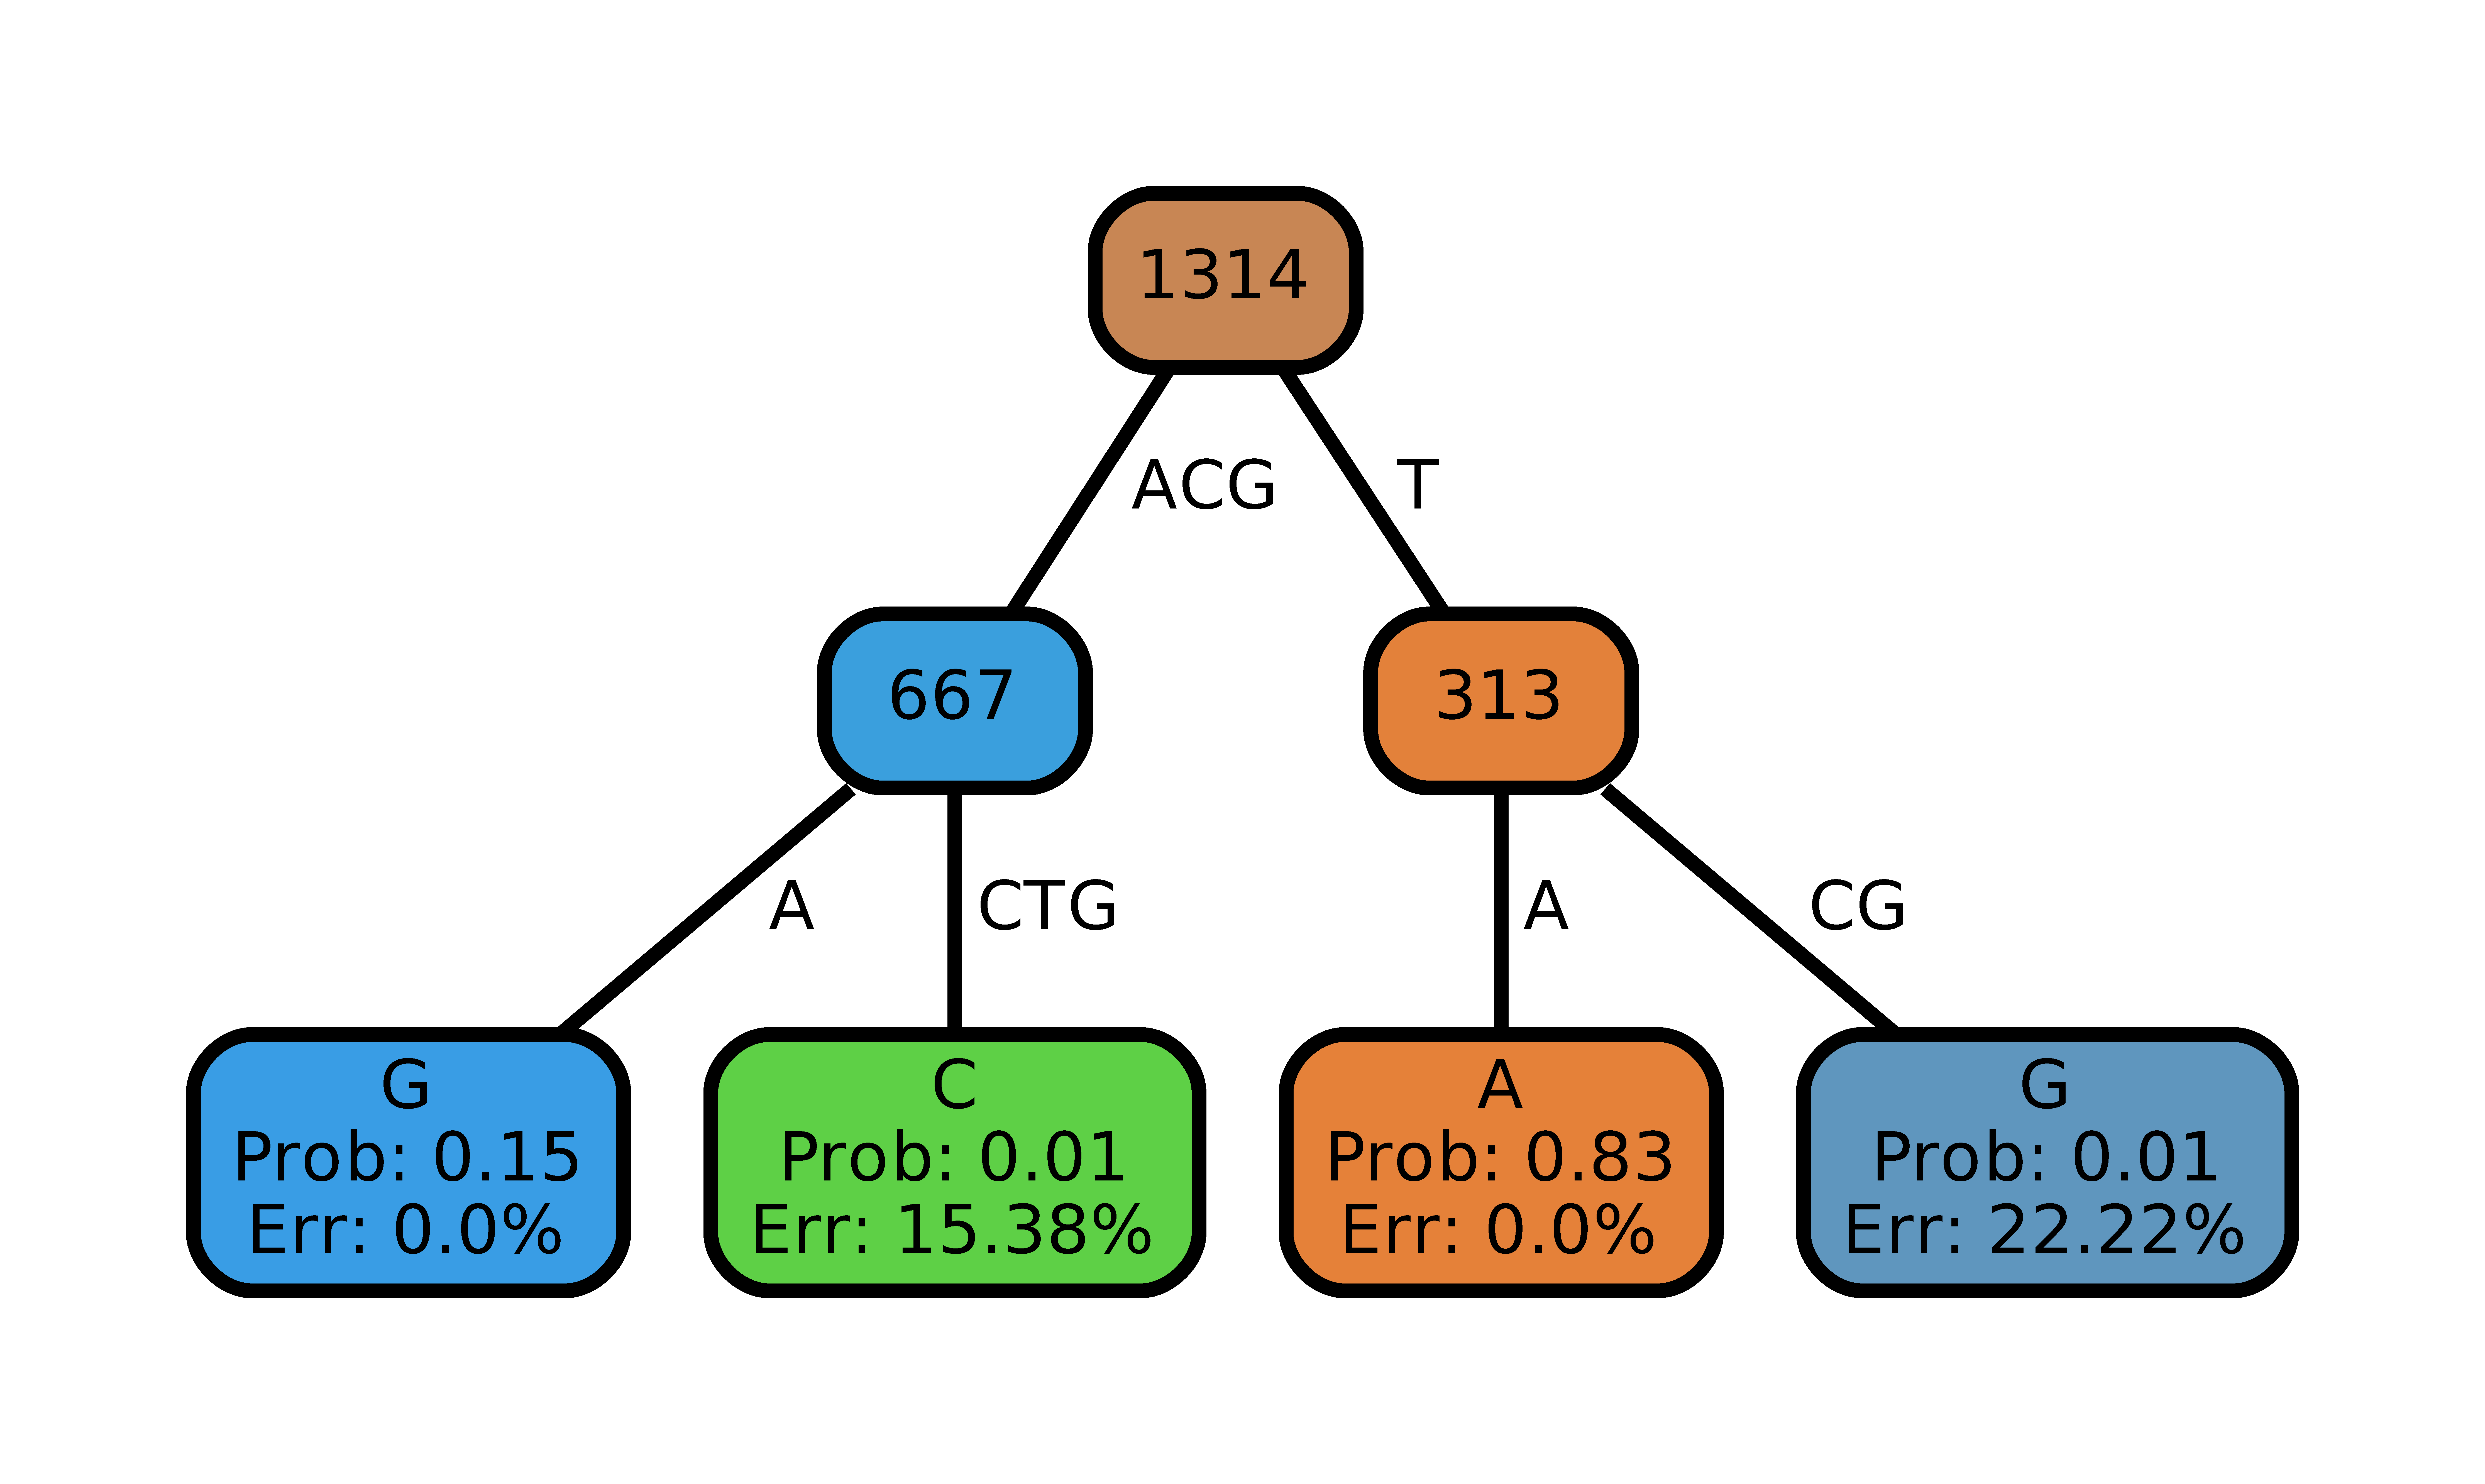
\includegraphics[width=\WDTD]{Figures/plotdata/TREE_P1263}};

\node[xcircs,inner sep=10.5pt] (N1) at ([yshift=.575in,xshift=.25in]P1274) {};
\node[xcircs,inner sep=11pt] (N2) at ([yshift=.985in,xshift=-0.27in]P1314) {};
\node[xcircs,inner sep=11pt] (N3) at ([yshift=.67in,xshift=0.4in]P1064) {};
\node[xcircs,inner sep=10.5pt] (N4) at ([yshift=.57in,xshift=0.2in]P1263) {};
    \draw [xdr,-{Latex[length=10mm]}] (N1) -- (P1064);
    \draw [xdr,,-{Latex[length=10mm]}] (N2) -- (P1263);
    \draw [xdr,,-{Latex[length=10mm]}] (N3) -- ([xshift=.8in]P1314.center);
    \draw [xdr,,-{Latex[length=10mm]}] (N4) to [out=145,in=90,looseness=1.45] (P1314);


 
\node[font=\bf\sffamily,anchor=east,rounded corners=3pt,align=center] (I1) at ([yshift=-.35in,xshift=-.1in]P1274.west) {Color\\key$^\bigstar$};

\node[font=\bf\sffamily,anchor=north,rounded corners=3pt,text width=.1in,text height=.1in,fill=Purple1,align=center] (I1) at (I1.south) {T};

\node[font=\bf\sffamily,anchor=north,rounded corners=3pt,text width=.1in,text height=.1in,fill=DarkOrange3!70,align=center] (I1) at (I1.south) {A};

\node[font=\bf\sffamily,anchor=north,rounded corners=3pt,text width=.1in,text height=.1in,fill=SeaGreen2,align=center] (I1) at (I1.south) {C};

\node[font=\bf\sffamily,anchor=north,rounded corners=3pt,text width=.1in,text height=.1in,fill=DodgerBlue2!80,align=center] (I1) at (I1.south) {G};

\node[font=\bf\sffamily\fontsize{4}{5},anchor=north west,align=left,text=gray] (I1) at ([yshift=-.1in,xshift=-.1in]I1.south west) {
{\large$^\bigstar$}Mixed colors represent\\distribution over different\\nucleotide outcomes
};


    \end{tikzpicture}
  };
\def\WDT{2.25in}
 \node[anchor=south west] (Nf1) at ([xshift=-.15in,yshift=-.35in]N1.south east) {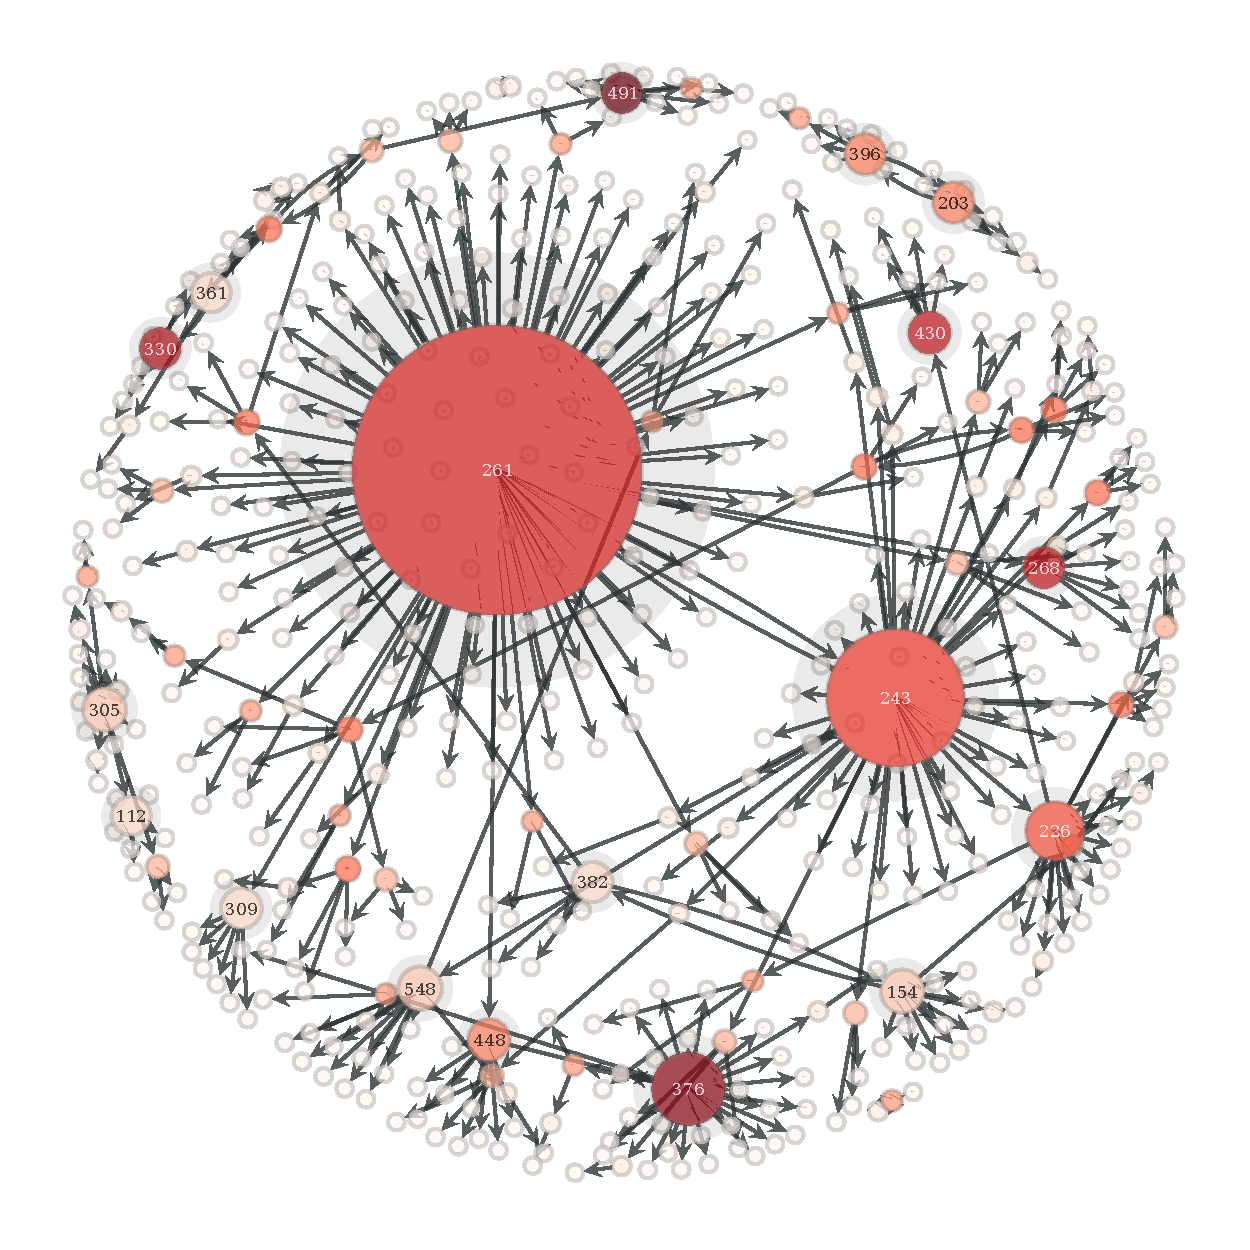
\includegraphics[width=\WDT]{Figures/qfig/output_human2009_2010}};

  \def\LWD{5pt}
  \node[anchor=north,align=left,font=\bf\tt\footnotesize] (N3) at ([yshift=-.1in,xshift=-0in]N1.south) {\bf\sffamily\fontsize{7}{8}\selectfont Influenza A 2018\\\bf\sffamily\fontsize{7}{8}\selectfont Haemagglutinin Sequences\\GGAAAACAAAAGCAACAAAA$\cdots$TGA{\large\color{Red1} A}AAAAGA$\cdots$CGCCAGTTCATTGGTACTGG\\AGCAAAAGCAGGGGAAAACA$\cdots $GTT{\large\color{Red1}C}AACCAC$\cdots$CTATTCAACTGCCGCCAGTT\\AGCAAAAGCAGGGGAAAACA$\cdots$GTT{\large\color{Red1}T}AACCAC$\cdots$CTATTCAACTGTCGCCAGTT\\ATGAAGACTATCATTGCTTT$\cdots$ACC{\large\color{Red1}T}TGAGAA$\cdots$GTGTTGCTTTGTTGGGGTTC};

\node[anchor=west,align=left,font=\bf\sffamily\fontsize{8}{10}\selectfont] (N4) at ([xshift=.2in]N3.east) {A/Italy/7366/2018\\
A/Baltimore/P0264/2018\\
A/Baltimore/P0278/2018\\  
A/Florida/61/2018};

\draw [ultra thick] ([yshift=.25in,xshift=.01in]N4.west) --++ (-.23in,-.19in);
\draw [ultra thick] ([yshift=.1in,xshift=.01in]N4.west) --++ (-.23in,-.2in);
 \draw [ultra thick] ([yshift=-0.05in,xshift=.01in]N4.west) --++ (-.23in,-.2in);
 \draw [ultra thick] ([yshift=-.2in,xshift=.01in]N4.west) --++ (-.23in,-.2in);

\draw [-{Latex[length=10mm]},ultra thick,line width=\LWD,\ACOL] ([xshift=-.1in,yshift=-.25in]N3.north) --++(0,.8in) node [yshift=-1.25in,below,align=center,text=IndianRed2] {residue\\1274};



\node[anchor=north west] (N11) at ([xshift=-.7in,yshift=.9in]N1.north east) {\begin{tikzpicture}
  \def\EQJ{$\geqq -C-C' \langle \theta \rangle$}
\clip (-.85in,-4.2in) rectangle (6.05in,1.35in);
\newcommand{\rgon}[1][black,loosely dashed,fill=lightgray,opacity=.4]{\tikz{ 
    \draw [thick,#1] 
    plot [smooth cycle, tension=1, domain=0:320, samples=28] (\x:{1.2+rand/10});
  }} 
\def\DCOL{black}

\def\COLB{black!20}
\def\TEXTCOL{black!100}

\def\COLB{black}
\def\TEXTCOL{gray}

\def\SCALE{.3}
    \node[align=center,label={[align=center,yshift=-0.3in,font=\bf\sffamily\fontsize{8}{8}\selectfont]90:Sequence Database\\\color{darkgray}NCBI, GISAID, $\cdots$},
circle,
line width=4pt,path fading=fade out,fill=black,inner sep=1pt,ball color=white,shading=ball] (N0) at (0,0) {
    \begin{tikzpicture}[rectangle,inner sep=0pt,rounded corners=0pt]
      %\clip (-.45in,-1in) rectangle (.75in,.15in);
    \node[] (A) at (0,0) {
      %\def\COLB{gray}
      %\def\TEXTCOL{black}
      \xdef\symbolstr{attatggacggatttagac}
\def\iX{10}
\begin{tikzpicture}[anchor=center,scale=\SCALE,text=\TEXTCOL,font=\sffamily\fontsize{7}{7}\selectfont, remember picture]
  % \useasboundingbox (-3.1,3) rectangle (4.75,.5); %all frames having the same size
  %\useasboundingbox (-3.5,-2) rectangle (25,6);
  % \node  [anchor=  west] (Q) at (-3.5,.75) {\BLACKBOX};

  \def\nuPi{3.1459265}
  \pgfmathtruncatemacro{\aaaa}{\iX-1}
  \pgfmathtruncatemacro{\bbbb}{\aaaa-1}
  \foreach \i in {\iX,\aaaa,...,0}{% This one doesn't matter
    \foreach \j in {1,0}{% This will crate a membrane
      % with the front lipids visible
      \pgfmathsetmacro{\dx}{rand*0.0}% A random variance in the x coordinate
      \pgfmathsetmacro{\dy}{rand*0.0}% A random variance in the y coordinate,
      % gives a hight fill to the lipid
      \pgfmathsetmacro{\rot}{rand*0.0}% A random variance in the
      \coordinate (A\i\j) at ({\i+\dx+\rot},{1*\j+\dy+0.6*sin(\i*\nuPi*20)});      
    }
  }
  \foreach \i in {\aaaa,\bbbb,...,1}{
    \StrChar{\symbolstr}{\i}[\symbol]
    \pgfmathtruncatemacro{\iminus}{\i - 1}
    \draw [thin, white,fill=\COLB, opacity=.85] (A\iminus0) -- (A\i0) -- (A\i1) -- (A\iminus1) -- cycle  ;
    \path (A\iminus0) -- (A\iminus1) node[midway] (N1) {};
    \path (A\i0) -- (A\i1) node[midway] (Nx\iX\i) {};
    \path (N1) -- (Nx\iX\i) node[midway] (N) {\bf \texttt \symbol} ;
  }%
  \pgfmathsetmacro{\dx}{\iX /3+.5 }
\end{tikzpicture}
};
    \node[anchor=north] (A) at ([xshift=.1in,yshift=.05in]A.south) {
      %\def\COLB{Red1!90}
      %\def\TEXTCOL{lightgray}
      \xdef\symbolstr{attatggacggatttagac}
\def\iX{10}
\begin{tikzpicture}[anchor=center,scale=\SCALE,text=\TEXTCOL,font=\sffamily\fontsize{7}{7}\selectfont, remember picture]
  % \useasboundingbox (-3.1,3) rectangle (4.75,.5); %all frames having the same size
  %\useasboundingbox (-3.5,-2) rectangle (25,6);
  % \node  [anchor=  west] (Q) at (-3.5,.75) {\BLACKBOX};

  \def\nuPi{3.1459265}
  \pgfmathtruncatemacro{\aaaa}{\iX-1}
  \pgfmathtruncatemacro{\bbbb}{\aaaa-1}
  \foreach \i in {\iX,\aaaa,...,0}{% This one doesn't matter
    \foreach \j in {1,0}{% This will crate a membrane
      % with the front lipids visible
      \pgfmathsetmacro{\dx}{rand*0.0}% A random variance in the x coordinate
      \pgfmathsetmacro{\dy}{rand*0.0}% A random variance in the y coordinate,
      % gives a hight fill to the lipid
      \pgfmathsetmacro{\rot}{rand*0.0}% A random variance in the
      \coordinate (A\i\j) at ({\i+\dx+\rot},{1*\j+\dy+0.6*sin(\i*\nuPi*20)});      
    }
  }
  \foreach \i in {\aaaa,\bbbb,...,1}{
    \StrChar{\symbolstr}{\i}[\symbol]
    \pgfmathtruncatemacro{\iminus}{\i - 1}
    \draw [thin, white,fill=\COLB, opacity=.85] (A\iminus0) -- (A\i0) -- (A\i1) -- (A\iminus1) -- cycle  ;
    \path (A\iminus0) -- (A\iminus1) node[midway] (N1) {};
    \path (A\i0) -- (A\i1) node[midway] (Nx\iX\i) {};
    \path (N1) -- (Nx\iX\i) node[midway] (N) {\bf \texttt \symbol} ;
  }%
  \pgfmathsetmacro{\dx}{\iX /3+.5 }
\end{tikzpicture}
};
    \node[anchor=north] (A) at ([xshift=.1in,yshift=.050in]A.south) {
     % \def\COLB{Red1!70}
      %\def\TEXTCOL{lightgray}
      \xdef\symbolstr{attatggacggatttagac}
\def\iX{10}
\begin{tikzpicture}[anchor=center,scale=\SCALE,text=\TEXTCOL,font=\sffamily\fontsize{7}{7}\selectfont, remember picture]
  % \useasboundingbox (-3.1,3) rectangle (4.75,.5); %all frames having the same size
  %\useasboundingbox (-3.5,-2) rectangle (25,6);
  % \node  [anchor=  west] (Q) at (-3.5,.75) {\BLACKBOX};

  \def\nuPi{3.1459265}
  \pgfmathtruncatemacro{\aaaa}{\iX-1}
  \pgfmathtruncatemacro{\bbbb}{\aaaa-1}
  \foreach \i in {\iX,\aaaa,...,0}{% This one doesn't matter
    \foreach \j in {1,0}{% This will crate a membrane
      % with the front lipids visible
      \pgfmathsetmacro{\dx}{rand*0.0}% A random variance in the x coordinate
      \pgfmathsetmacro{\dy}{rand*0.0}% A random variance in the y coordinate,
      % gives a hight fill to the lipid
      \pgfmathsetmacro{\rot}{rand*0.0}% A random variance in the
      \coordinate (A\i\j) at ({\i+\dx+\rot},{1*\j+\dy+0.6*sin(\i*\nuPi*20)});      
    }
  }
  \foreach \i in {\aaaa,\bbbb,...,1}{
    \StrChar{\symbolstr}{\i}[\symbol]
    \pgfmathtruncatemacro{\iminus}{\i - 1}
    \draw [thin, white,fill=\COLB, opacity=.85] (A\iminus0) -- (A\i0) -- (A\i1) -- (A\iminus1) -- cycle  ;
    \path (A\iminus0) -- (A\iminus1) node[midway] (N1) {};
    \path (A\i0) -- (A\i1) node[midway] (Nx\iX\i) {};
    \path (N1) -- (Nx\iX\i) node[midway] (N) {\bf \texttt \symbol} ;
  }%
  \pgfmathsetmacro{\dx}{\iX /3+.5 }
\end{tikzpicture}
};
    \node[anchor=north] (A) at ([xshift=-.1in,yshift=.05in]A.south) {
     % \def\COLB{Red1!80}
      %\def\TEXTCOL{lightgray}
      \xdef\symbolstr{attatggacggatttagac}
\def\iX{10}
\begin{tikzpicture}[anchor=center,scale=\SCALE,text=\TEXTCOL,font=\sffamily\fontsize{7}{7}\selectfont, remember picture]
  % \useasboundingbox (-3.1,3) rectangle (4.75,.5); %all frames having the same size
  %\useasboundingbox (-3.5,-2) rectangle (25,6);
  % \node  [anchor=  west] (Q) at (-3.5,.75) {\BLACKBOX};

  \def\nuPi{3.1459265}
  \pgfmathtruncatemacro{\aaaa}{\iX-1}
  \pgfmathtruncatemacro{\bbbb}{\aaaa-1}
  \foreach \i in {\iX,\aaaa,...,0}{% This one doesn't matter
    \foreach \j in {1,0}{% This will crate a membrane
      % with the front lipids visible
      \pgfmathsetmacro{\dx}{rand*0.0}% A random variance in the x coordinate
      \pgfmathsetmacro{\dy}{rand*0.0}% A random variance in the y coordinate,
      % gives a hight fill to the lipid
      \pgfmathsetmacro{\rot}{rand*0.0}% A random variance in the
      \coordinate (A\i\j) at ({\i+\dx+\rot},{1*\j+\dy+0.6*sin(\i*\nuPi*20)});      
    }
  }
  \foreach \i in {\aaaa,\bbbb,...,1}{
    \StrChar{\symbolstr}{\i}[\symbol]
    \pgfmathtruncatemacro{\iminus}{\i - 1}
    \draw [thin, white,fill=\COLB, opacity=.85] (A\iminus0) -- (A\i0) -- (A\i1) -- (A\iminus1) -- cycle  ;
    \path (A\iminus0) -- (A\iminus1) node[midway] (N1) {};
    \path (A\i0) -- (A\i1) node[midway] (Nx\iX\i) {};
    \path (N1) -- (Nx\iX\i) node[midway] (N) {\bf \texttt \symbol} ;
  }%
  \pgfmathsetmacro{\dx}{\iX /3+.5 }
\end{tikzpicture}
};
  \end{tikzpicture}};
%\node[single arrow, minimum width=1in,fill=lightgray, path fading=west,minimum height=.6in,anchor=north,align=center,text=black!60] (A1) at ([yshift=-.5in]N0.south) {Machine\\Learning};
\node[anchor=north,label={[align=center,yshift=0.05in,xshift=-.25in,font=\bf\sffamily\fontsize{8}{8}\selectfont]90:Infer Constraints\\\color{gray}(\qnet construction)},] (N1x) at ([xshift=-0in,yshift=-.5in]N0.south) {
  \def\COLB{black}
\def\TEXTCOL{gray}
  \def\SCALE{.45}
      %\def\TEXTCOL{lightgray}
  \xdef\symbolstr{attatggacggatttagac}
\def\iX{10}
\begin{tikzpicture}[anchor=center,scale=\SCALE,text=\TEXTCOL,font=\sffamily\fontsize{7}{7}\selectfont, remember picture]
  % \useasboundingbox (-3.1,3) rectangle (4.75,.5); %all frames having the same size
  %\useasboundingbox (-3.5,-2) rectangle (25,6);
  % \node  [anchor=  west] (Q) at (-3.5,.75) {\BLACKBOX};

  \def\nuPi{3.1459265}
  \pgfmathtruncatemacro{\aaaa}{\iX-1}
  \pgfmathtruncatemacro{\bbbb}{\aaaa-1}
  \foreach \i in {\iX,\aaaa,...,0}{% This one doesn't matter
    \foreach \j in {1,0}{% This will crate a membrane
      % with the front lipids visible
      \pgfmathsetmacro{\dx}{rand*0.0}% A random variance in the x coordinate
      \pgfmathsetmacro{\dy}{rand*0.0}% A random variance in the y coordinate,
      % gives a hight fill to the lipid
      \pgfmathsetmacro{\rot}{rand*0.0}% A random variance in the
      \coordinate (A\i\j) at ({\i+\dx+\rot},{1*\j+\dy+0.6*sin(\i*\nuPi*20)});      
    }
  }
  \foreach \i in {\aaaa,\bbbb,...,1}{
    \StrChar{\symbolstr}{\i}[\symbol]
    \pgfmathtruncatemacro{\iminus}{\i - 1}
    \draw [thin, white,fill=\COLB, opacity=.85] (A\iminus0) -- (A\i0) -- (A\i1) -- (A\iminus1) -- cycle  ;
    \path (A\iminus0) -- (A\iminus1) node[midway] (N1) {};
    \path (A\i0) -- (A\i1) node[midway] (Nx\iX\i) {};
    \path (N1) -- (Nx\iX\i) node[midway] (N) {\bf \texttt \symbol} ;
  }%
  \pgfmathsetmacro{\dx}{\iX /3+.5 }
\end{tikzpicture}

};
\draw[very thick,  dashed,\DCOL] ([xshift=.05in]N1x.center) -- ++(.5in,0.5in) node[circle,fill=none] (XX1){} -- ++(.1in,-0.35in);
\draw[very thick, dashed,\DCOL] ([xshift=-.15in,yshift=-.1in]N1x.center) -- ++(-.25in,-0.5in) node[circle,fill=none] (XX){} -- ++(-.25in,0.6in);
\draw[very thick, dashed,\DCOL] (XX.center) -- ++(1.2in,.570in);

%\node[single arrow, minimum width=1in,fill=lightgray, path fading=west,minimum height=.6in,anchor=west,align=left,text=black!50] (A2) at ([xshift=-.15in]N1x.east) {Biologically\\meaningful\\distance};
\node[anchor=north,label={[]-90:Biology-aware q-distance},font=\bf\sffamily\fontsize{22}{14}\selectfont] (N2) at ([xshift=0.1in,yshift=-.7in]N1x.south) {
 $\theta\left ({x},{y}\right )$};
\draw[-stealth', ultra thick,Red1] (N1x) -- ++(0,-.85in);
\draw[-stealth', ultra thick,Red1] ([yshift=.25in]N0.south) -- ++(0,-.35in);
\end{tikzpicture}

};




  \node[anchor=south west,align=left] (L1) at ([xshift=-4in,yshift=-.55in]N1.north west) {{\Large a.} Portion of Recursive Forest Underlying Q-Net\\Inferred for Human Influenza A HA 2018-19 Season};
  \node[anchor=west,align=left] (L2) at ([xshift=.75in]$(L1.west)!(N0.north west)!(L1.east)$) {{\Large b.} Construction of q-distance};
  \node[anchor=south west,align=left] (L3) at ([yshift=-.15in]$(L2.north west)!(Nf1.north west)!(L2.south west)$) {{\Large c.} Human Influenza A HA 2008-9{\Large$^\dag$}\\(Coinciding Swine Flu Pandemic 2009)};

\node[draw=black!2,very thick, rounded corners=5pt, anchor=north west,align=left,font=\bf\sffamily\fontsize{8}{7}\selectfont,text=IndianRed2] (LLL) at ([yshift=-1.6in,xshift=-1in]L3.south west) {\mnp{.75in}{\raggedright {\large$^\dag$}Denser color\\ \& size implies more  edges}};
%  \node[anchor=west,align=left] (L2) at ([xshift=.75in,yshift=-4in]$(L1.west)!(N0.north west)!(L1.east)$) {{\Large C.} Q-Net Domains:\\Swine Influenza A HA 2018-19 season};

  
\end{tikzpicture}
